\documentclass{article}
\title{Projet de fin d'études}
\author{Ian Gruson}
\date{Janvier 2021}

\usepackage{float}
\usepackage{graphicx}
\usepackage{hyperref}
\usepackage{color}
\usepackage{listings}
\usepackage{pdfpages}
\usepackage[francais]{babel}
\usepackage{varioref}
\usepackage{minted}

\begin{document}
\maketitle
\begin{center}
	\large\textbf{Tuteur de stage : Patrick Bard}\\
	\vspace*{\stretch{1.0}}
	\large\textbf{Enseignant référant : Jérôme Rossignol}

\end{center}
\vspace*{\stretch{1.0}}
\begin{center}
	\large\textbf{ESIREM}\\
	
\includegraphics[scale=0.7]{images/logoEsirem}\\
	\vspace*{\stretch{1.0}}
	\large\textbf{Promotion Pascal}
	\vspace*{\stretch{1.0}}\\
	\large\textbf{LEAD}\\
	\large\textbf{Intitulé de la mission : Développement d'un générateur de figures de Navon}
\end{center}
\vspace*{\stretch{2.0}}
\newpage
\renewcommand{\contentsname}{Sommaire}
\tableofcontents
\newpage
\renewcommand{\listfigurename}{Liste des figures}
\listoffigures
\newpage
\section{Remerciements}
J'aimerais remercier les professeurs de l'ESIREM pour leurs enseignements au travers de ces trois années d'école. En particulier je voudrais remercier M. Sergey Kirgizov pour sa pédagogie, sa bienveillance et son souci du bien-être de ses étudiants. Suivre ses cours fut toujours un plaisir.

\newpage
\section{Présentation de l'entreprise}
Le Laboratoire d'étude de l'apprentissage et du développement (LEAD) est un laboratoire de recherche axé sur la psychologie cognitive basé à Dijon. Le Laboratoire étudie les spécificités de l'apprentissage autant implicite qu'explicite et les influences d'un environnement sur ce dernier. Le laboratoire étudie plus particulièrement les processus cognitifs impliqués dans la lecture, l'écriture, l'apprentissage d'une langue ou encore de la musique. Le laboratoire dispose de matériel sophistiqué tel que des oculomètres, ou des ElectroEncéphaloGraphes (EEG) pour réaliser des expériences de haut vol. Le laboratoire fait parti de l'Institut des Sciences Biologiques (INSB) du Centre National de Recherche Scientifique (CNRS).  

\section{Mission du stage}
Un des test sur l'apprentissage implicite et explicite très connu dans le monde de la psychologie cognitive est le test des figures de Navon (fig : \ref{fig:figure_Navon}) créer par David N. Une figure de Navon est classiquement une lettre de l'alphabet, formé à partir d'une autre lettre de l'alphabet plus petite. Par exemple, on dessine une grande lettre T (que l'on appelle communément la figure globale) à partir de petites lettres b (les lettres locales). Le test consiste à montrer à un candidat une série de figures de Navon auquel il doit répondre rapidement en indiquant la figure locale qu'il voit. Le test n'est évidemment pas simple car par réflexe le candidat aura plutôt tendance à se focaliser sur la figure globale.
Pour effectuer un test, il convient d'avoir un nombre de figures important et varié afin d'avoir des résultats plus fiables. Or, à ce jour, il n'existe pas d'outils permettant de générer de façon simple et rapide ces figures, et les chercheurs du LEAD sont contraints de les créer à la main sur un tableur. 
La mission de ce stage était de produire un logiciel simple d'utilisation qui permettait aux chercheurs de générer une multitudes de figures rapidement et de façon configurable. Le choix de la méthode de génération était libre, du moment que l'application permettait de configurer un certain nombre de paramêtres bien spécifiques. La figure doit pouvoir être configurable par sa forme (figure globale), sa figure locale, la taille de la figure locale, la taille de la figure globale, et sa densité. La densité correspond à l'espacement entre les lettres locales. Une formule de la densité à été donné par M. Bard comme étant une analogie à la loi des gaz parfaits : \label{formule:equation_densité}\[d = n * t / T\] où d est la densité, n le nombre de lettres locales, t la taille lettres locales et T la taille de la figure globale. En admettant que l'utilisateur fixe d, t et T, alors n est déterminé par le générateur. Un figure moins dense comportera alors moins de figures locales.


\begin{figure}[!h]
	\centering
	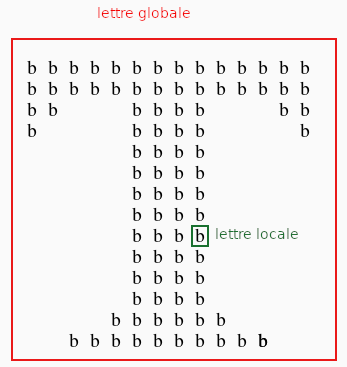
\includegraphics[scale=0.6]{./images/figureT.png}
	\caption{example d'une figure de Navon avec comme figure globale un T et comme figure locale un b}
	\label{fig:figure_Navon}
\end{figure}

\newpage
\section{Précédents travaux}
La mission a été confié à un autre étudiant en DUT l'année passée, et l'approche qui avait été privilégié était de configurer les figures à partir de fichiers json contenant des points en coordonnées cartésiennes. Ces points permettaient ensuite de tracer les lettres locales suivant des droites. Pour un A il faut 5 points représentant 5 sommets pour tracer trois droites.


\section{Approche actuelle}
\subsection{génération des figures}
L'approche qui fut développé dans ce travail, consistait à utiliser des listes de 0 et de 1 (bitmap) pour former les lettres globales (fig : \ref{fig:bitarray}). La taille de la liste correspond à la résolution de la figure de Navon. Pour chaque 1 dans la liste, le générateur imprime un caractère ou une lettre, et pour chaque zéro, il n'imprime rien. La taille des listes étant bien évidemment modifiable, il est possible des créer des formes plus ou moins complexes. 

\begin{figure}[!h]
	\centering
	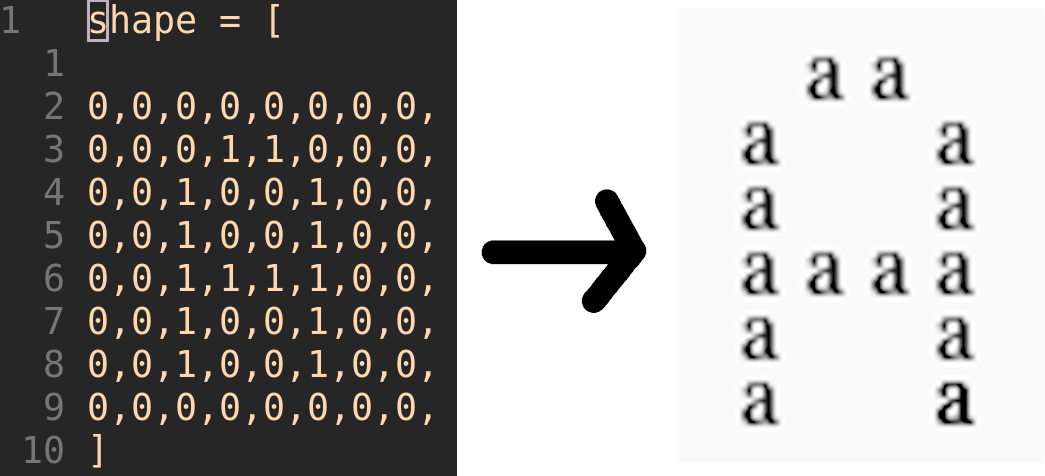
\includegraphics[scale=0.9]{./images/txt_to_image.png}
	\caption{exemple d'un bitmap d'une figure représentant un A majuscule}
	\label{fig:bitarray}
\end{figure}

\subsection{génération des bitmap}

En partant de cette base pour générer des figures, il faut encore pouvoir générer les bitmap rapidement et sans difficultés afin de simplifier la tâche des psychologues. La création d'une application graphique pour ordinateur était donc nécessaire. L'application a été développé en C++ avec l'API Qt. Cette combinaison de technologies permet une grande portabilité sur différents systèmes d'exploitation (Windows, Linux et MacOS) grâce au C++, et une grande modularité dans la création des widgets graphiques avec Qt. 

Le principe de l'application est d'afficher un canevas sur lequel l'utilisateur peut venir dessiner ses figures de Navon, et génerer des fichiers texte contenant les bitmap. Il pourra par la suite générer les images à partir de ces fichiers à l'aide d'un bouton sur l'interface. 
L'idée du canevas pour dessiner les figures s'inspire des applications comme Piskel (fig:\ref{fig:Piskel}) qui permettent de créer des sprites de jeux vidéos en pixel art (8bits, 16 bits, 32 bits, etc...). Cette manière de dessiner a pour avantage son extrême simplicité d'utilisation et de prise en main, et s'accorde parfaitement aux bitmaps qui sont générés.

\begin{figure}[!h]
	\centering
	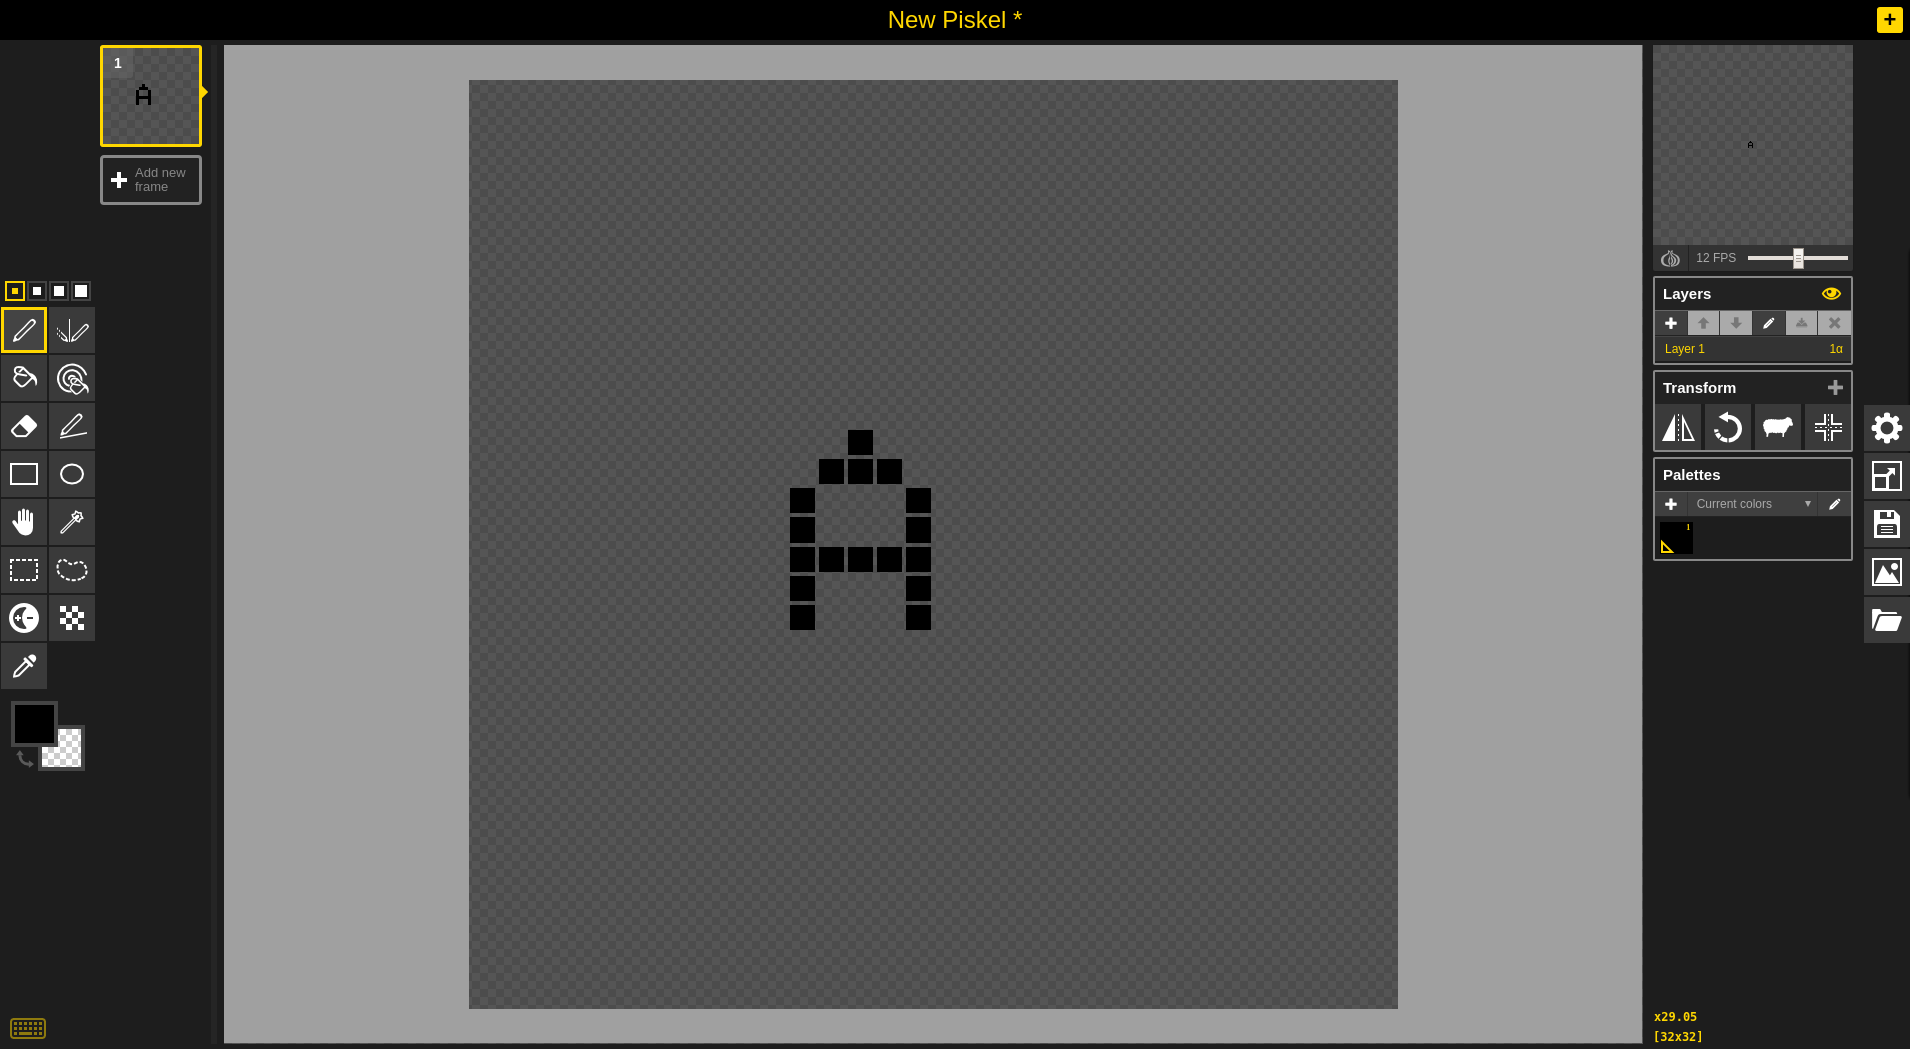
\includegraphics[scale=0.2]{./images/piskel.png}
	\caption{interface de l'application Piskel}
	\label{fig:Piskel}
\end{figure}

Comme pour Piskel, l'application affiche un canevas sur lequel l'utilisateur peut cliquer et afficher des carrés noirs. Pour chaque carrés noirs affichés sur le canevas, un bit passera un 1 dans le bitmap au même index (fig : \ref{fig:canevas_array}). 

\begin{figure}[!h]
	\centering
	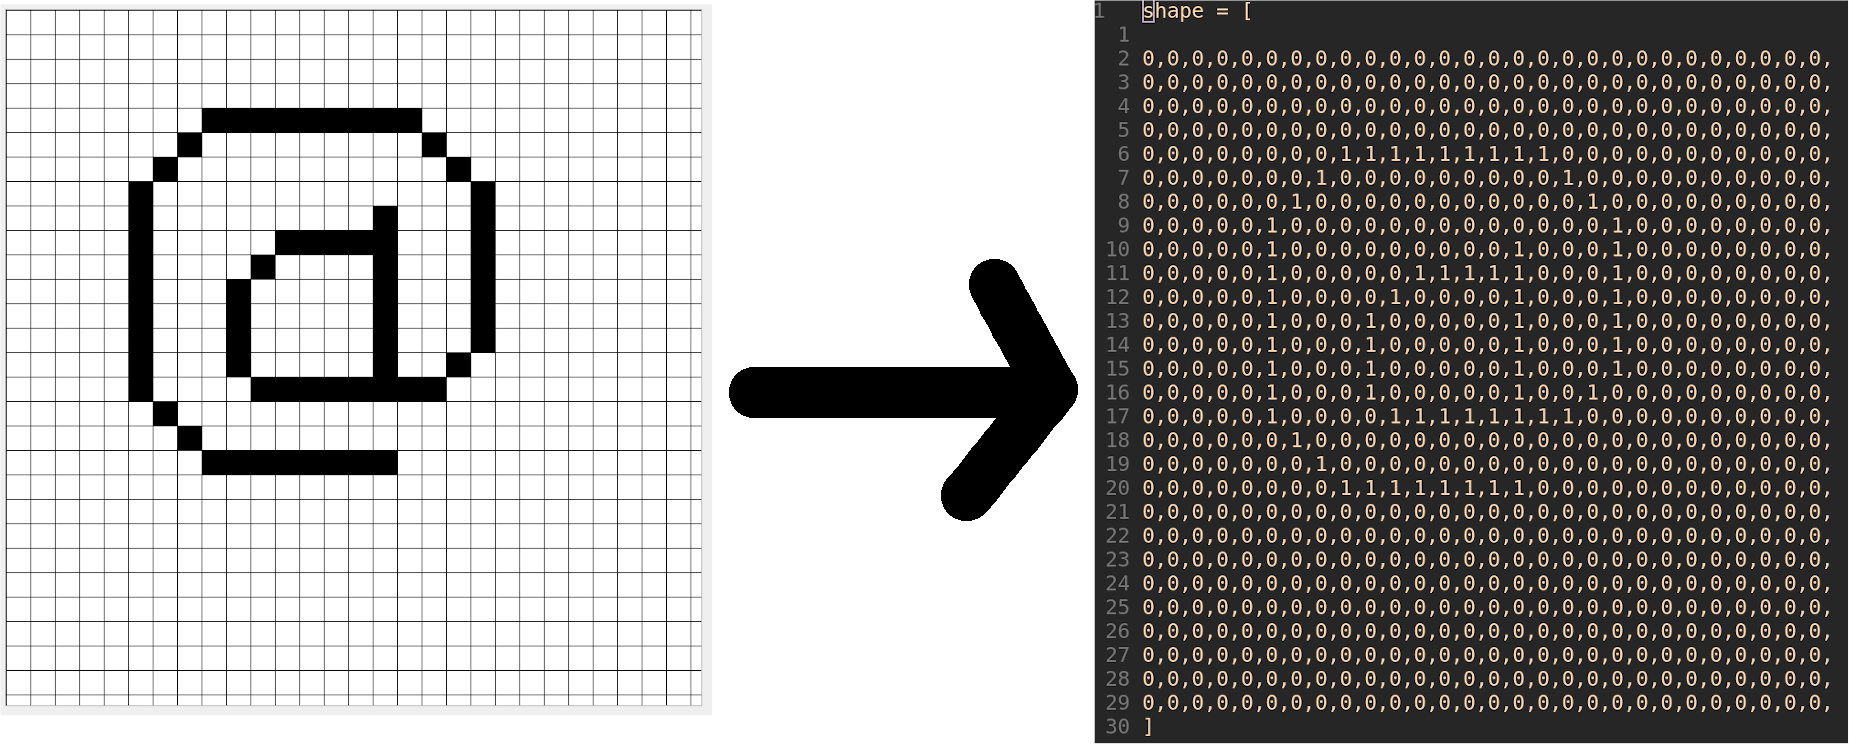
\includegraphics[scale=0.8]{./images/grid-txt.png}
	\caption{exemple de la génération du bitArray depuis la grille}
	\label{fig:canevas_array}
\end{figure}

\newpage
\section{Diagramme UML}
\subsection{Diagramme cas d'utilisation}

L'application devra suivre ce diagramme d'utilisation fig:\ref{fig:utilisation}. L'utilisateur peut dessiner la figure sur l'interface et modifier les paramètres de génération de l'image. La génération de l'image par l'application dépend de la construction des fichiers texte. Et le contenu des fichiers texte dépendent des dessins de l'utilisateur. D'autres fonctionnalités pourraient être ajoutées par la suite afin d'aller plus loin dans le confort d'utilisation et la flexibilité d'édition. 

\begin{figure}[!h]
	\centering
	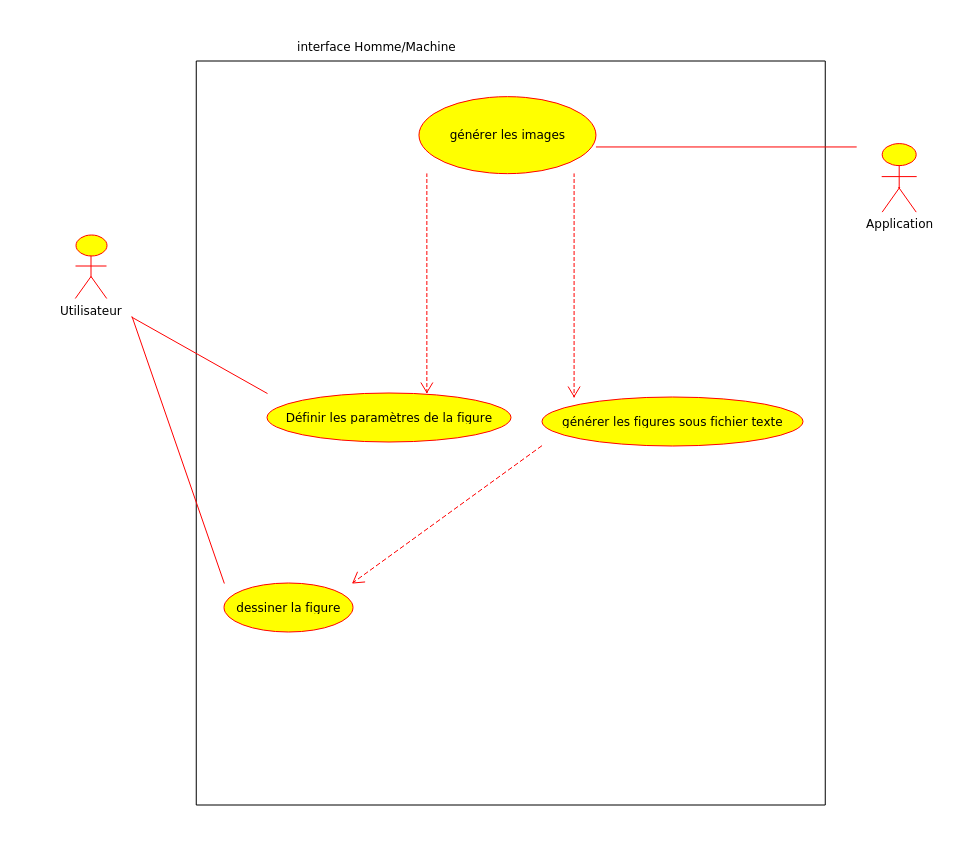
\includegraphics[scale=0.35]{./images/diagramme_cas_utilisation.png}
	\caption{diagramme de cas d'utilisation du générateur.}
	\label{fig:utilisation}
\end{figure}

\newpage
\subsection{Diagramme de classes}
Le diagramme de classes du générateur est le suivant (fig : \ref{fig:classe_figure}). Le constructeur de la classe navonFigure prend le caractère local, la taille de police et l'espacement pour gérer la densité des caractères. La classe gridCanvas, qui affiche le canevas sur lequel l'utilisateur peut dessiner ses figures, comporte trois attributs : canvasWidth (la taille du canvas en pixel), sizeOfCell (la taille d'une case/cellule), et numberOfCells (le nombre de cases/cellules, soit la résolution de la grille).

\begin{figure}[!h]
	\centering
	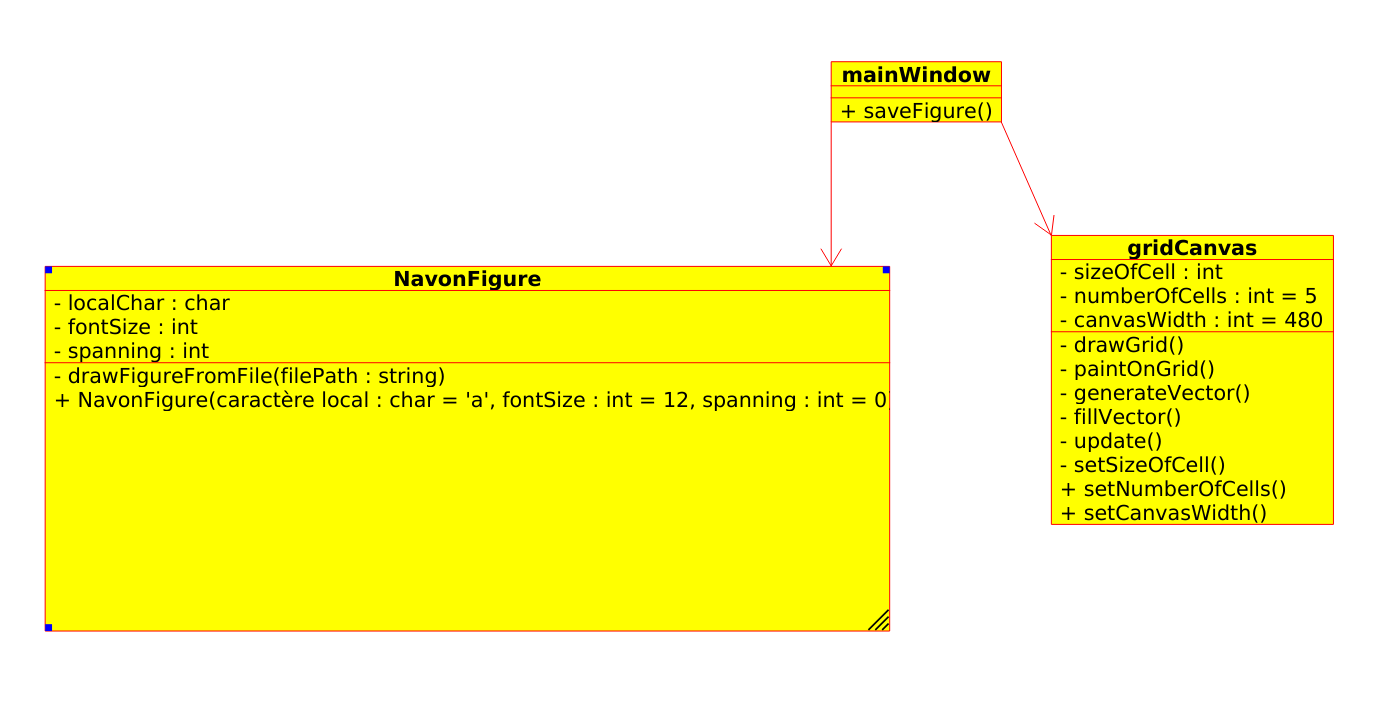
\includegraphics[scale=0.25]{./images/diagramme_classe.png}
	\caption{diagramme de classes du générateur}
	\label{fig:classe_figure}
\end{figure}

\newpage
\section{Présentation de l'application}
\subsection{Générateur des bitmaps}
La figure \ref{fig:interface} correspond à l'interface de l'application telle qu'elle est à ce jour. L'utilisateur est face à la grille de dessin et dispose de quelques boutons et slider. Toute la partie gauche de l'interface est consacrée à la grille et à la génération des fichiers texte. Il y a deux sliders : le premier permet d'agrandir ou de rétrécir la zone de dessin, tandis que le deuxième modifie le nombre de cases/cellules de la grille. Les sliders réinitialisent également le canevas et les bitmaps car le code ne comporte pas encore de fonctions permettant de conserver et d'adapter les carrés noir déssinés et le bitmap aux changements des propriétés du canevas. L'utilisateur devra donc changer les propriétés du canevas selon ses envies avant de commencer à dessiner. Ensuite, il y a un bouton "create .txt file" qui permet à l'utilisateur de choisir le chemin du fichier texte correspondant au bitmap et de le générer. 

\subsection{Générateur d'images}
La partie droite de l'application se concentre sur la génération des images à partir des fichiers texte. L'utilisateur choisit d'abord le fichier texte contenant la (ou les) figure(s) de Navon, puis il choisit les paramètres (taille de police, espacement entre les lettres, et caractère local). Pour le moment, la densité est gérée en espaçant ou en rapprochant les figures locales avec une valeur en pixel, et ne tient pas compte de la formule de densité énoncé page \pageref{formule:equation_densité}. Enfin il peut générer son image en cliquant sur le bouton "generate image" qui ouvrira un explorateur de fichier, où il devra spécifier le chemin du fichier texte correspondant à son image.

\subsubsection{code source de la génération d'images}
\begin{minted}[obeytabs=true,tabsize=4]{c++}
void NavonFigure::drawFigureFromFile(string filepath, QString imagePath)
{
	fstream figureFile;
	vector<int> globalShape;
	string line;
	bool figureStored = false;
	int figureNum=0;
	int arrIndex=0;
	figureFile.open(filepath,ios::in);
	if(figureFile.is_open()){
		while(!figureFile.eof()){
			getline(figureFile,line, '\n');
			for(int i =0; i<line.size(); i++){
				char c[] = {line[i]};
				if(c[0] == '1' || c[0] == '0'){
					globalShape.push_back(stoi(c));
					arrIndex++;
				}
				//given that each shape arrays end with a ] in the txt file 
				//we reset the arrIndex to 0
				//to rewrite globalShape with the next shape.
				if(c[0]==']')
				{
					figureStored = true;
				}
			}
			if(figureStored)
			{
				arrIndex=0;
				int i;
				QChar local_char = this->character;
				QImage image(960, 960, QImage::Format_RGB32);
				image.fill(QColor(250,250,250));
				QPainter painter(&image);
				painter.setFont(QFont("Times",fontSize));
				QPoint topLeft(0,0);
				QPoint bottomRight(fontSize, fontSize);
				QRect rect(topLeft, bottomRight);
				for(i=0; i<globalShape.size(); i++){
					if(i%int(sqrt(globalShape.size())) == 0)
					{
						topLeft.setX(0); topLeft.setY(topLeft.y()+fontSize+spanning);
						bottomRight.setX(fontSize+spanning);
						bottomRight.setY(bottomRight.y()+fontSize+spanning);
					}
					if(globalShape[i] == 1)
					{
						rect.setTopLeft(topLeft); rect.setBottomRight(bottomRight);
						painter.drawText(rect, Qt::AlignCenter, local_char);
					}
					topLeft.setX(topLeft.x()+fontSize+spanning);
					bottomRight.setX(bottomRight.x()+fontSize+spanning);
				}
				bool isSaved = image.save(imagePath, "PNG", 100);
			}
		}
	}
	else{
	}
	figureFile.close();
}
\end{minted}
Cette fonction permet de créer les images des figures. Chaque caractére est imprimé sur l'image grâce à un objet QRect qui englobe un seul caractère, dans lequel on appelle la méthode drawText si il y a un 1 dans le vecteur globalShape avec des coordonnées topLeft et bottomRight. En parcourant le vecteur globalShape l'objet QRect est déplacé en modifiant les coordonnées topLeft et bottomRight. Lorsqu'une ligne est terminée, QRect retourne à la ligne et continu. De plus la variable spanning gère l'espacement en pixel et modifie les coordonnées topLeft et bottom. Dans l'interface, l'utilisateur peut rentrer une valeur négative pour rapprocher les lettres, ou une valeur positive pour espacer les lettres. Enfin l'image est sauvegardée en png avec une qualité de 100, c'est à dire en une image de meilleure qualité non compressée. À noter que la fonction conserve des des aspects qui prenait en compte le fait qu'un fichier texte comporte plusieurs figures. Plus dans le projet cette fonction pouvait créer plusieur images d'où la présence des lignes comme : 
\begin{minted}{c++}
	if(c[0]==']')
	{
		figureStored = true;
	}
\end{minted}
Qui vérifie qu'une figure a bien été complétement stocké dans le vecteur globalShape et que l'image peut être imprimée. 


\begin{figure}[!h]
	\centering
	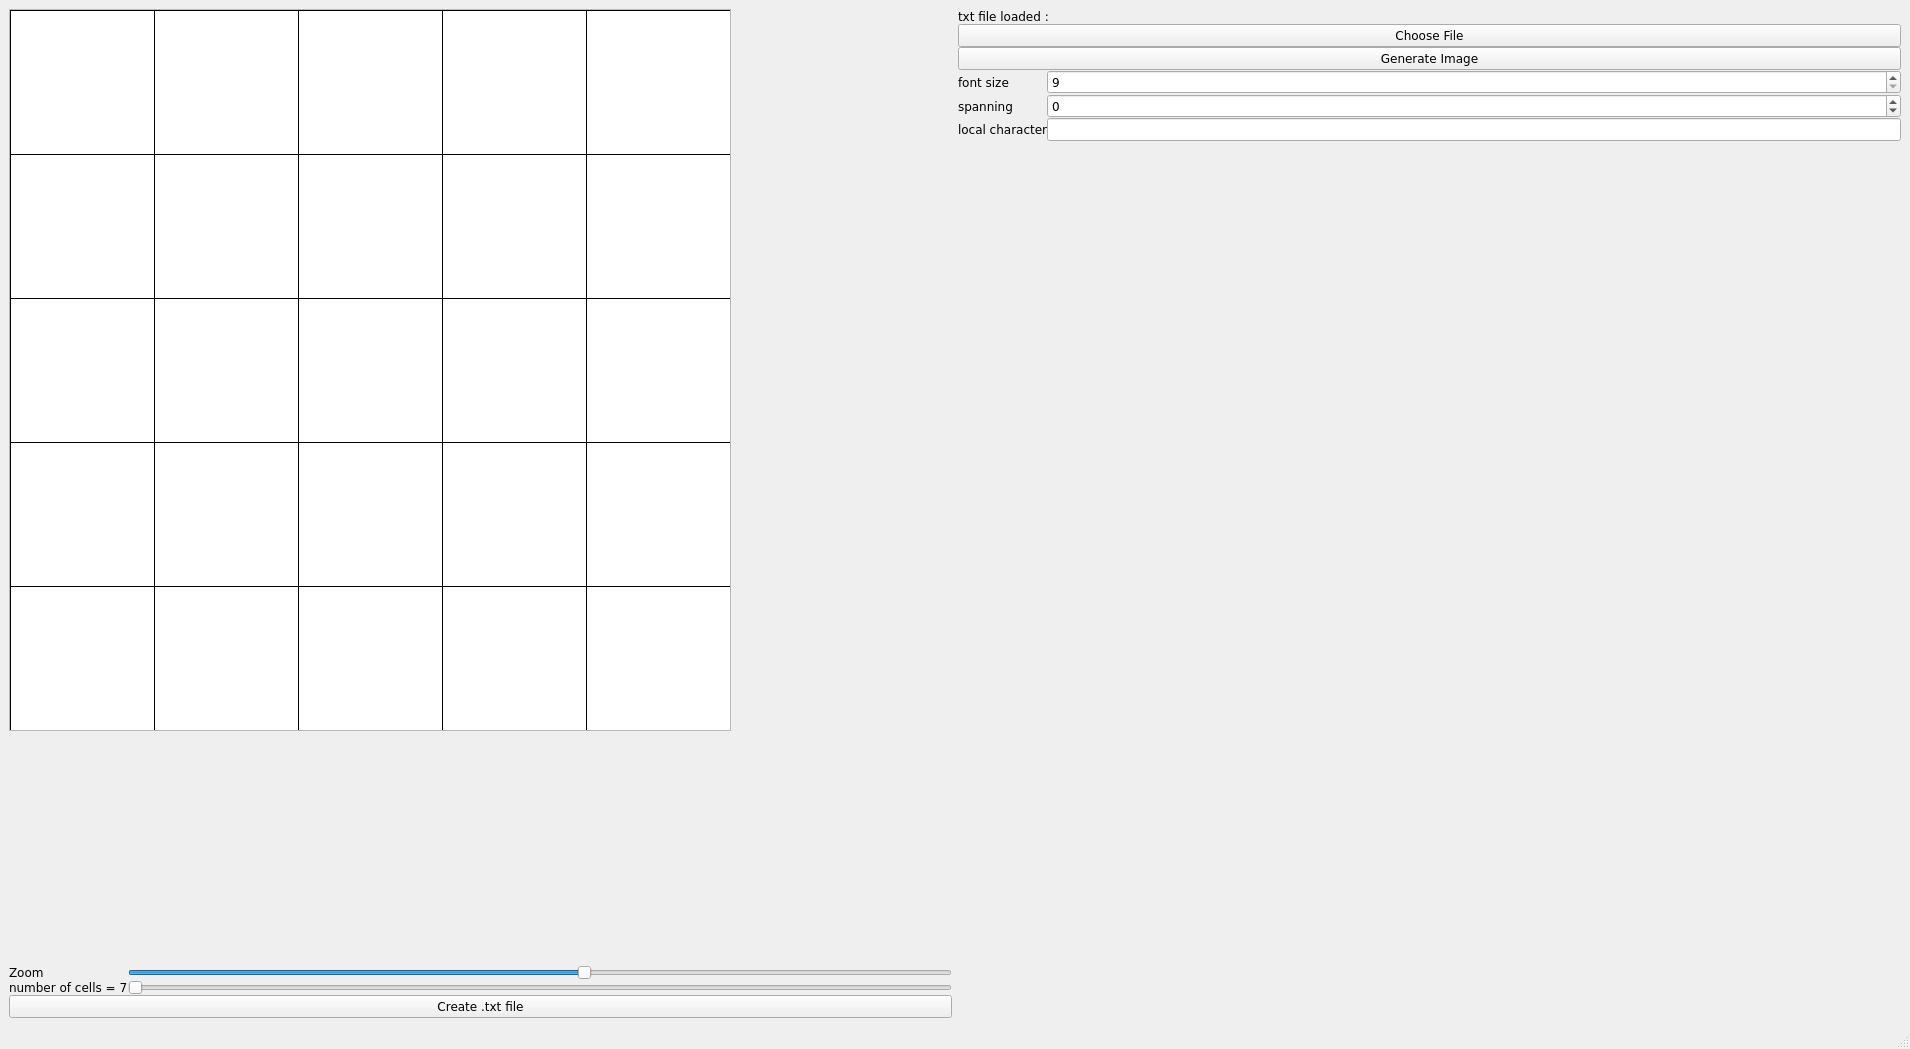
\includegraphics[scale=0.2]{./images/interface.png}
	\caption{interface de l'application}
	\label{fig:interface}
\end{figure}

\section{Création d'un exécutable Windows}
\subsection{M Cross Environment}
Une tâche de la mission était de créer un éxecutable Windows indépendant de toutes librairies pour facilter l'usage du logiciel. En effet compiler des logiciels à la main n'est pas facile et amusant pour les non-initiés donc cette étape était importante pour le projet. Le logiciel a été développé et compilé sous Ubuntu et Arch Linux qui sont des distributions GNU/Linux, donc il marche également sous ces systèmes d'exploitation. L'éxecutable Windows a été crée en utilisant M Cross Environment (MXE) qui est un Makefile GNU qui compile des programmes pour différents environnements. Son utilisation est plutôt simple il suffit de se placer dans le répertoire du projet Qt contenant le fichier .pro et de saisir la comande /usr/lib/mxe/usr/x86\_64-w64-mingw32.static/qt5/bin/qmake generateur\_de\_figures.pro sous Linux puis la commande make. Un dossier release est alors créer contenant l'éxecutable generateur\_de\_figures.exe qui est un éxecutable pour les architectures 64 bits.

\section{Application}
En plus d'aider les chercheurs du LEAD dans leur travail, cette application pourra profiter à d'autres pyschologues à travers le monde. En effet, plusieurs options sont envisageables : l'application pourrait être publiée en open-source sur des platerformes telles que github ou gitlab, ou être vendue sous la forme d'éxecutable. La publication de l'application en open source pourrait être particulièrement bénéfique pour ce type de projet. En effet, des améliorations et des corrections pourraient être apportées par des contributeurs, ainsi les pyschologues du LEAD pourraient profiter de ces améliorations.

\section{Conclusion}
Pour conclure, l'application est fonctionnelle, et dessiner les figures sur la grille est simple et rapide même avec énormément de cases. Cette approche possède une limite néanmoins : il n'est pas possible de dessiner des courbes ou des cercles. La meilleure façon d'approcher des courbes est d'augmenter le nombre de cases et les dessiner à la main. Une résolution suffisante de cases peut aisément donner l'impression de courbures. Bien que l'application soit utilisable, elle mériterait néamoins d'être améliorée et peaufinée. En effet, quelques fonctionnalités pourraient être ajoutées pour augmenter son intérêt. La plus évidente est la possibilité de recharger le dessin sur la grille à partir d'un fichier texte existant pour modifier une figure. À ce jour, pour effectuer des petites modifications sur une figure il faut le modifier directement dans le fichier texte. 

Sur le plan personnel, créer cette application de toutes pièces fut instructif. J'ai pu mieux prendre en main Qt et j'ai réussi à franchir le pic de difficulté initial. En effet, Qt est un framework extrêmement dense et puissant et comprendre le fonctionnement des différents objets qu'il propose réprésente un investissement important. J'ai néanmoins trouvé ce projet motivant car j'ai du faire preuve de créativité pour arriver à ce résultat. De plus, créer des programmes informatiques reste toujours un plaisir pour moi. 

\newpage
\section{Bibliographie}
Des tentatives de recherches ont été faites, et bien que les figures de Navon ont vu bien des papiers scientifiques écrits à leurs sujet, rien en lien avec de la génération ou l'informatique n'a été trouvé. Aucun papier scientifique n'a été utilisé pour produire l'application et rédiger ce rapport.

Seule mention à Piskel qui est open-source, qui m'est utile lorsque je développe des jeux vidéos en pixel art et qui m'a servi d'inspiration pour le canevas de l'application.
Piskel https://www.piskelapp.com/
Site de MXE : https://mxe.cc/
Site du LEAD : http://leadserv.u-bourgogne.fr/fr/

\end{document}
